\subsection{Time series components touched - For packages touched for  each week commit} 
\begin{figure}
  \centering 
  \begin{subfigure}[b] 
{0.45\textwidth}
    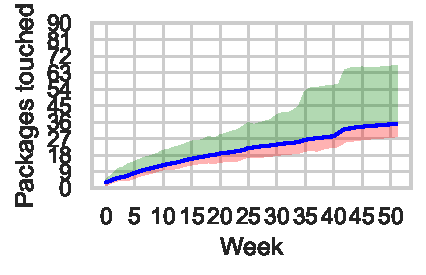
\includegraphics{sections/results/packages/time_series_components_touched.packages.all.founders.week_52.pdf}
    \caption{Packages for All founders (n=34, $\mu$=35.38, median=14.0 \& std=23.11)}
    \label{figure.sections/results/packages/time_series_components_touched.packages.all.founders.week_52.pdf}
  \end{subfigure}
  \begin{subfigure}[b] 
{0.45\textwidth}
    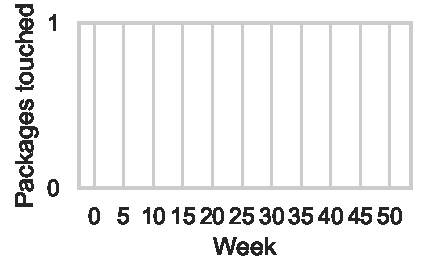
\includegraphics{sections/results/packages/time_series_components_touched.packages.all.joiners.week_52.pdf}
    \caption{Packages for All joiners (n=203, $\mu$=35.84, median=13.0 \& std=33.4)}
    \label{figure.sections/results/packages/time_series_components_touched.packages.all.joiners.week_52.pdf}
  \end{subfigure}
\newpage 
  \begin{subfigure}[b] 
{0.45\textwidth}
    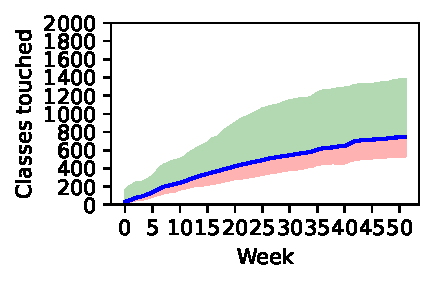
\includegraphics{sections/results/classes/time_series_components_touched.classes.all.founders.week_52.pdf}
    \caption{Classes for All founders (n=34, $\mu$=746.15, median=321.28 \& std=515.17)}
    \label{figure.sections/results/classes/time_series_components_touched.classes.all.founders.week_52.pdf}
  \end{subfigure}
  \begin{subfigure}[b] 
{0.45\textwidth}
    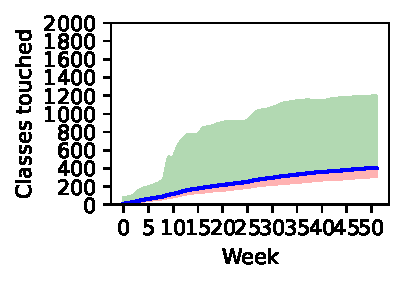
\includegraphics{sections/results/classes/time_series_components_touched.classes.all.joiners.week_52.pdf}
    \caption{Classes for All joiners (n=203, $\mu$=408.05, median=125.0 \& std=440.63)}
    \label{figure.sections/results/classes/time_series_components_touched.classes.all.joiners.week_52.pdf}
  \end{subfigure}
\newpage 
  \begin{subfigure}[b] 
{0.45\textwidth}
    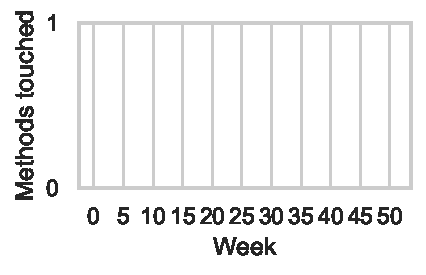
\includegraphics{sections/results/methods/time_series_components_touched.methods.all.founders.week_52.pdf}
    \caption{Methods for All founders (n=34, $\mu$=3129.0, median=1296.71 \& std=2539.1)}
    \label{figure.sections/results/methods/time_series_components_touched.methods.all.founders.week_52.pdf}
  \end{subfigure}
  \begin{subfigure}[b] 
{0.45\textwidth}
    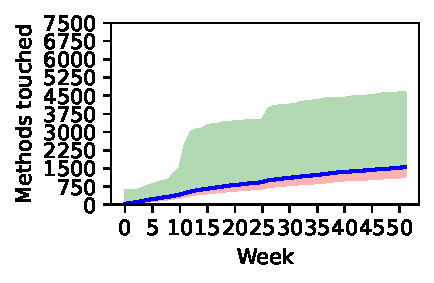
\includegraphics{sections/results/methods/time_series_components_touched.methods.all.joiners.week_52.pdf}
    \caption{Methods for All joiners (n=203, $\mu$=1545.61, median=435.2 \& std=1709.56)}
    \label{figure.sections/results/methods/time_series_components_touched.methods.all.joiners.week_52.pdf}
  \end{subfigure}
\caption{A time series for the all commits, excluding transient, with the average mean (blue line), all components touched (y-axis) against the number of week (x-axis) for two (2) developer categories. Green is the standard deviation above the mean, and pink is the standard deviation below the mean.}\end{figure}
\clearpage 
\newpage 
